\documentclass{beamer}
\usetheme{default} 

%\setbeamertemplate{background canvas}[vertical shading][bottom=green!3,top=green!10] 
%\setbeamercolor{structure}{fg=OliveGreen!50!black} 
\usebackgroundtemplate{
    \centering
\includegraphics[width=\paperwidth,height=\paperheight]{images/android_wall}
}

\usepackage[utf8x]{inputenc}
\usepackage{default}
\usepackage{listings}

\lstset{language=java, basicstyle=\small, commentstyle=\color{gray}}
\lstset{frame=single}

\title{Android - Podstawy}
\author{Konrad Malawski \\ konrad.malawski@java.pl}

\begin{document}

\begin{frame}
\titlepage
\end{frame}

\begin{frame}
\frametitle{Architektura}

  \begin{figure}[t]
    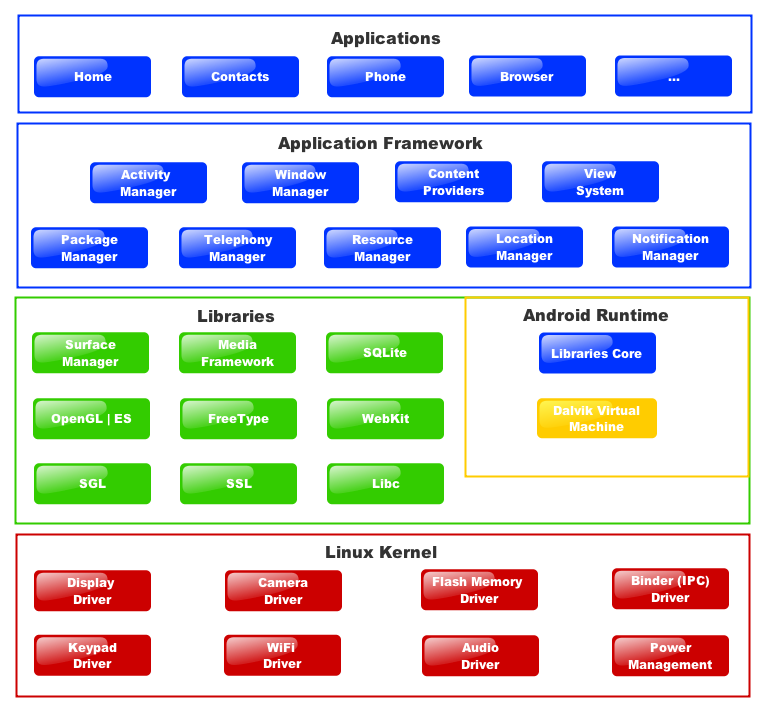
\includegraphics[height=0.62\textheight,keepaspectratio=true,clip=true,trim=0 0 0 100]{images/platform}
    \caption{Architektura systemu Android}
  \end{figure}

\end{frame}

\begin{frame}
  \frametitle{It's Linux}
\begin{itemize}
 \item Warto pamiętać, Android = Linux (zawiera glibc etc)
\end{itemize}

\end{frame}

\begin{frame}[fragile]
\frametitle{Activity}
\begin{lstlisting}
  public class MainActivity extends Activity {
    public void onCreate(Bundle savedState) {
      /**/
    }
  }
\end{lstlisting}

\end{frame}


\end{document}
